\section{System Architecture}
%Describe the system architecture and its components.  Smap, Streamfs, mobile phones, qr codes, wireless acme meters.
%\emph{Mobile phone as the triple-point!!!}
Our architecture consists of various components, with the mobile phone serving as the centerpiece.  Smart phones
serves as a point of intersection between the user, her environment, and compontational infrastructure.  Smarts phones
are highly personalized, are carried by users everywhere, and with ubquitous, multi-modal forms of accessing a network,
provide almost continuous access to services.  However, although space and context are nebulous ideas and difficult to capture
we can learn from user feedback.  In order to truly bridge the physical world to the virtual world, we include the use
of QR codes to tag \emph{any item the user finds relevant to capture}.  QR codes are easy to generate and inexpensive
to produce and replace.

With energy tracking as the main goal, we used QR codes to tag items that consume energy.  When an item is tagged, the user swipes
the tag and enters information about the item.  After this `registration phase' is complete, any user can use
their smart phone to learn about the item by swiping the QR code that is attached to it.  In addition to arbitrary
descriptive metadata, we distinguish between regular items and \emph{meters}.  Meters are items that produce
continuous energy data.  Meters are bound to items that are attached to them and serve as a proxy for the energy information
about the device it is attached to.  We describe how \emph{binding} between items is done in section~\ref{sec:binding}.
Figure~\ref{fig:sysarch} shows our system architecture and each of the components.

%FILL IN WITH REAL GRAPH
\begin{figure*}[htb!]
\begin{center}
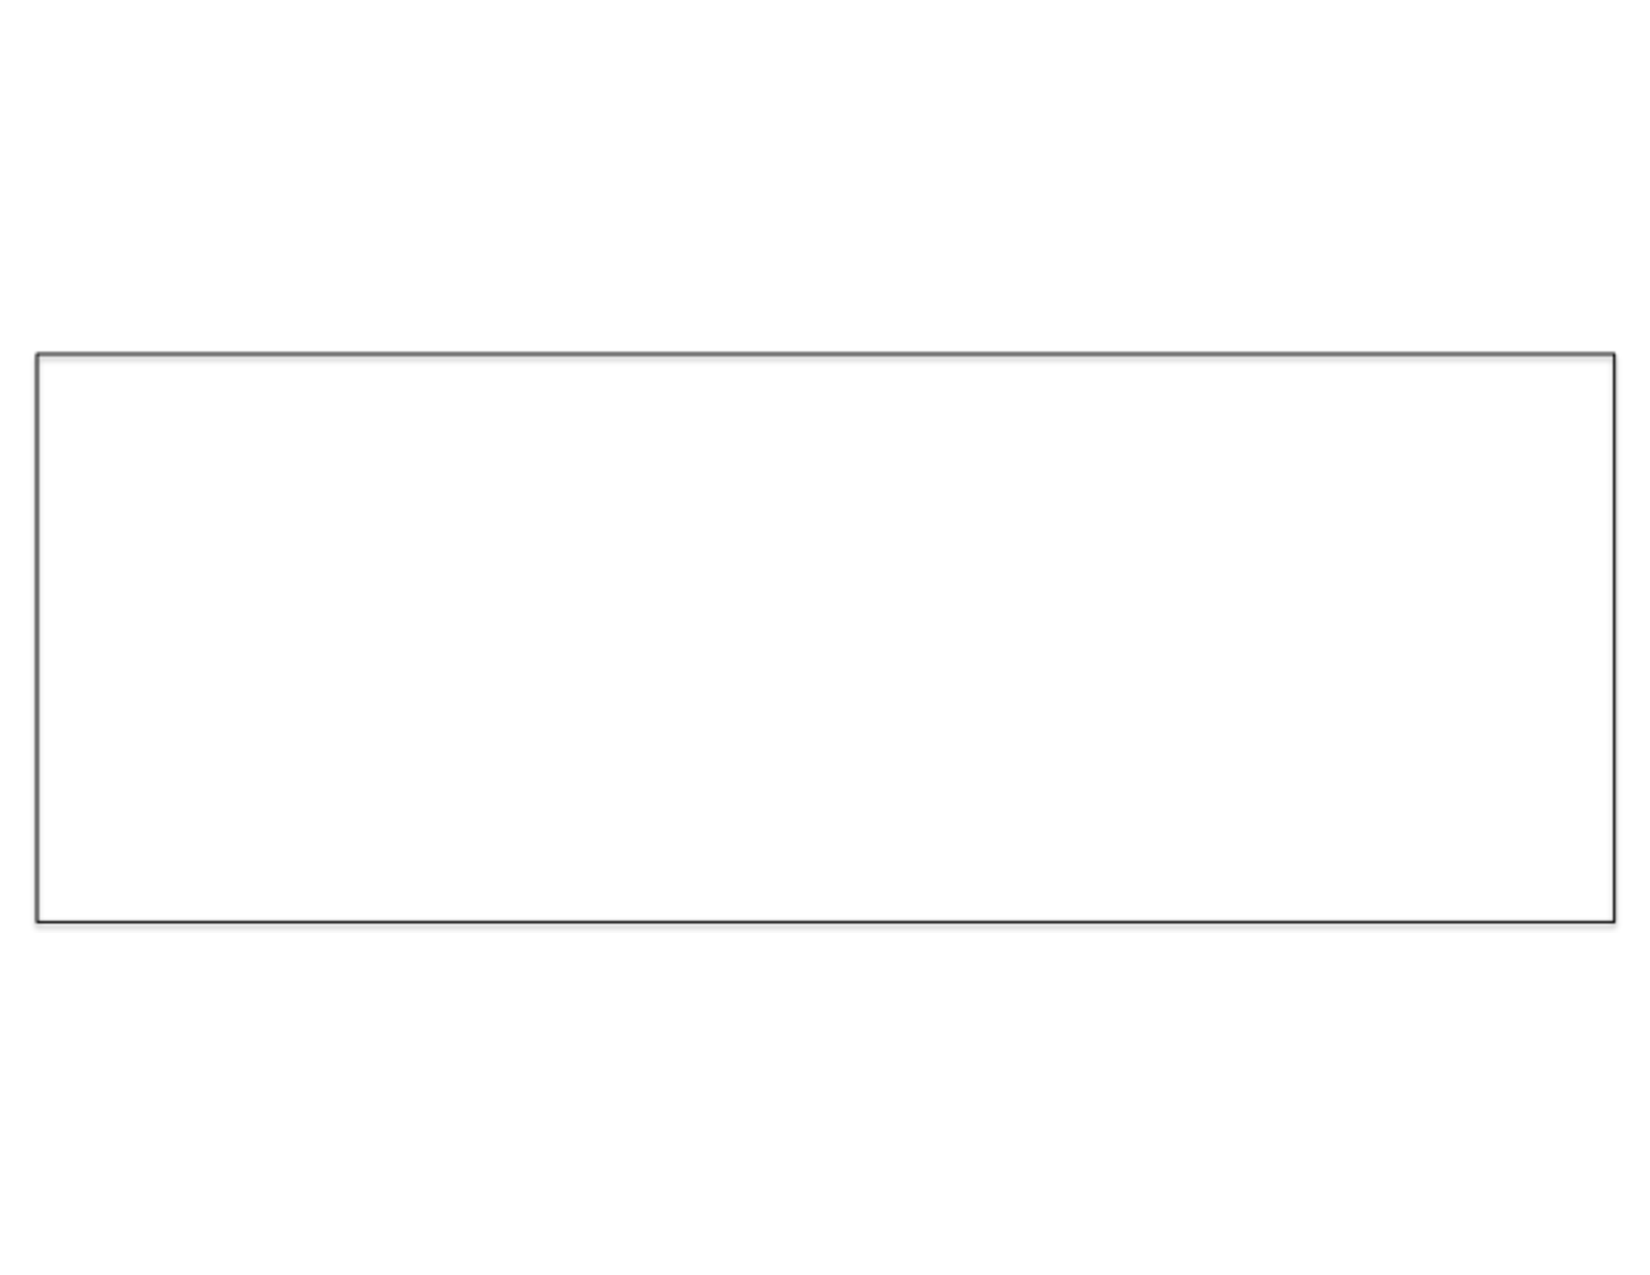
\includegraphics[scale=0.5]{figs/blankrectangle}
\caption{Architecture. Lorem Ipsum is simply dummy text of the printing and typesetting industry. Lorem Ipsum has 
been the industry's standard dummy text ever since the 1500s, when an unknown printer took a galley of 
type and scrambled it to make a type specimen book.  }
\label{fig:sysarch}
\end{center}
\end{figure*}

\subsection{Mobile phone}
\label{sec:mobilephone}
The mobile phone is at the center of our architecture.  Its basic function is to swipe QR codes in the environment,
do a lookup to the backend through the network, query for any relevant information to display to the user and display it.
Interaction with the user is through this set of displays.  For example, if a user wish to learn more about when
their television was on, they swipe the QR code on the television.  The phone offers various services that the television
provides.  In the current set of application we have written, you would get to read the description, make, and model of the
television.  You might also learn what the rated power of the television, if that was included in the metadata capture.
If the television has a meter attached and that meter is virtually and physically bound to it, on of our applications
also allows you to view the power traces associated with television over various time intervals.  The default is 24-hours.

\subsection{QR Codes}
\label{sec:qrc}
A QR code is a two-dimensional barcode.  You may encode up to almost 3000 bytes of data on them.  QR code generators
can be found on the internet~\cite{qrcgen1, qrcgen2}.  We encoded a lookup {\tt URL} that our applications use to
direct users to the appropriate web address and to identify the specific item that the QR code was attached to.

% \begin{figure}[htb!]
% \begin{center}
% 
\includegraphics[scale=0.3]{figs/qrcex}
% \caption{This is an example QR code from our application. This label resolves to {\tt http://tinyurl.com/6235eyw}.
% We used tinyUrl to reduce the QR code image complexity and scan time.}
% \label{fig:qrcex}
% \end{center}
% \end{figure}

% \begin{figure}[htb!]
% \begin{center}
% 
\includegraphics[scale=0.125]{figs/qrcexlong}
% \caption{This is an example QR code from our application. This label resolves to {\tt http://tinyurl.com/6235eyw}.
% We used tinyUrl to reduce the QR code image complexity and scan time.}
% \label{fig:qrcex}
% \end{center}
% \end{figure}

\begin{figure}[htb!]
\label{fig:qrcex}
\begin{center}
\subfigure[Long QR Code.]{%
            \label{fig:qrcexfirst}
            
\includegraphics[scale=0.148]{figs/qrcexlong}
        }
\subfigure[Minimized QR Code.]{%
            \label{fig:qrcexsecond}
            
\includegraphics[scale=0.35]{figs/qrcex}
        }
\end{center}
\caption{
	The QR code on the left resolves to the same {\tt URL} at the right one, after resolution and
	redirection is complete. 
	The short label resolves to {\tt http://tinyurl.com/6235eyw}.
	We used tinyUrl to reduce the QR code image complexity and scan time.
     }%
\end{figure}

An interesting observation we made in our deployments is that complex QR codes are difficult to capture and resolve
quickly, especially under poor lighting conditions.
The more data you encode on the QR code, the more 
intricate the pattern that is generated, therefore we tried to minimize the size of the {\tt URL} encoded on the QR code.  
The examples above show the difference between encoding a 
long %~\footnote{{\tt http://is4server.com/mobile/nokia/mobile.php?qrc=4eb46a8709e57}}
{\tt URL} to a short {\tt URL} shows an % http://tinyurl.com/6235eyw}.  Figure~\ref{fig:qrcexsecond} shows an 
example QR code that we used to tag items in one of our deployments.  Notice the difference between Figures~\ref{fig:qrcexfirst} 
and \ref{fig:qrcexsecond}.  Since the first QR code is not only more complex, but also longer to scan
than the second.  

Table~\ref{tab:qrscans} shows the results of some simple scanning experiment between the two tags
shown above.  We scanned each QR code under light and dark lighting conditions, off the screen of my laptop.
Each experiment was run 10 times and the table shows the statistical overview of the results.  The absolute times
are less important than the relative times.  Clearly, scanning the simple QR code under well-lit conditions
performed the best.  In fact, the complex QR code under the same condition takes about 75\% longer to scan.
More importantly, however, is the variance.  Notice that the variance with the simple QR code is much smaller and
more stable under either condition.  In our experience, {\bf large variance in scan time is a major
problem for complex QR codes}.  That is why we decided to re-design them and push more information in the lookup
processes, as network access was more reliable than the focus of the camera on various mobile devices.
Tags are placed on all types of devices in all kinds of locations with varying degrees of lighting.
Simple QR codes are vital for widespread use as a physically tagging mechanism.

\begin{table}
\label{tab:qrscans}
\begin{center}
  \begin{tabular}{| r | c  c | }
    \hline
    			 & {\bf Average (sec) } & {\bf Variance (sec)} \\ \hline
    Short,light & 1.66 & 0.33 \\ \hline
    Short, dark & 2.08 & 0.35 \\ \hline
    Long, light & 2.26 & 0.71 \\ \hline
    Long, dark & 2.82 & 0.50 \\
    \hline
  \end{tabular}
\caption{Shows the time to scan a long QR code versus a short QR code in light and dark conditions (loosely defined).
Notice that short QR codes scan faster and with less variance that long ones.}
\end{center}

\end{table}


\subsection{Data infrastructure}
The third piece of our architecture consists of a data collection and management components.  The subcomponents
of this part of the archictecture are set up in layered fashion.  The context and data mangement layer is at the top,
the meter-access layer is below that, and at the bottom is the metering infrastructure.  The context layer sets up
a structured metadata organization whose semantics are interpretted by each application.  We describe the single structure
that supports our applications.  In addition, this layer unifies the metadata and the data, allowing the application
to access all meters data that share similar properties (i.e. placement, type, owner, etc.).  The meter data-access layer 
unifies the various access standards into a single interface.  This allows us to add sensors and easily incorporate it
into our context layer.  Finally, we integrated various types of meter data.  Specifically, we used several wireless
power meters called ACmes~\cite{acme} as well as various streams from the building management system directly.

\subsubsection{StreamFS}
\label{sec:streamfs}
%Discuss namespace management, binding, and recording data.
We used StreamFS~\cite{streamfs} as our data management layer.  StreamFS offers various
facilities to manage streaming sensor data and the associated metadata in a way that was useful for our the needs
of our application.  It organizes the metadata hierarchically and provides analytical
facilities that are fully baked into the system, making it easier to create energy-analytics applications.  In particular,
StreamFS deals well with data aggregation where the number of constituents used to calculate the aggregate
changes over time.  In StreamFS, this is called \emph{dynamic aggregation} and it is described in more detail
in section~\ref{sec:dynagg}.

Each object in physical space is represented by a node in StreamFS.  Through StreamFS' RESTful/HTTP interface, we can
fetch the any node through a path rooted at the location where StreamFS is hosted.  For example, if we wish
to access the power meter in room 400, we may access it by issuing an HTTP {\tt GET} request to
{\tt http://server.streamfs.com/bldg/rm400/pow}.  The request returns a {\tt JSON} object with attribute-value
pairs that give a description of the temperature sensor.  It also returned that last received value from that sensor.
StreamFS provides a query interface to fetch the timeseries data collected from the sensor as well.

In addition, StreamFS support symbolic linking and this allows us to refer to nodes by multiple names.  That same 
power meter can also be referred to through {\tt /jortiz/meters/pow}; the meters that belong to user \emph{jortiz}.
More generally, StreamFS offers features that simplify namespace and data management.  Semantically, the hierarchical
node structure can be interpretted by the application.  We describe the structure and interpretation in
each application is section~\ref{sec:apps}.

\subsubsection{sMAP}
\label{sec:smap}
%Disucss how the streaming meter data is forwarded to streamfs and linked to streamfs objects.
sMAP~\cite{smap} provides a uniform data access layer for sensor information.  We can take any of the various sensor protocols
and make it accessible through sMAP's HTTP, RESTful API.  In addition, sMAP servers can live on any machine that is accessible
through the web.  This is convenient for our purposes, since it makes the raw sensor data stream accessible through any network.
sMAP's data-forwarding facility is extensively to link the sensor data with the context layer.  When a meter is being added
to the context layer, a callback is installed on the sMAP server that hosts that meter's stream.  As meter data is reported 
to the sMAP server, it is forwarded to the appropriate node {\tt URL} in StreamFS, setting up the context associated with that
meter automatically.

\subsection{Metering layer}
We used several types of meter data in our applications.  Specifically we integrated the whole-building building power-draw feed,
and a number of feeds from our wireless ACme power-meter deployment.

%FILL IN WITH REAL GRAPH
\begin{figure*}[htb!]
\begin{center}
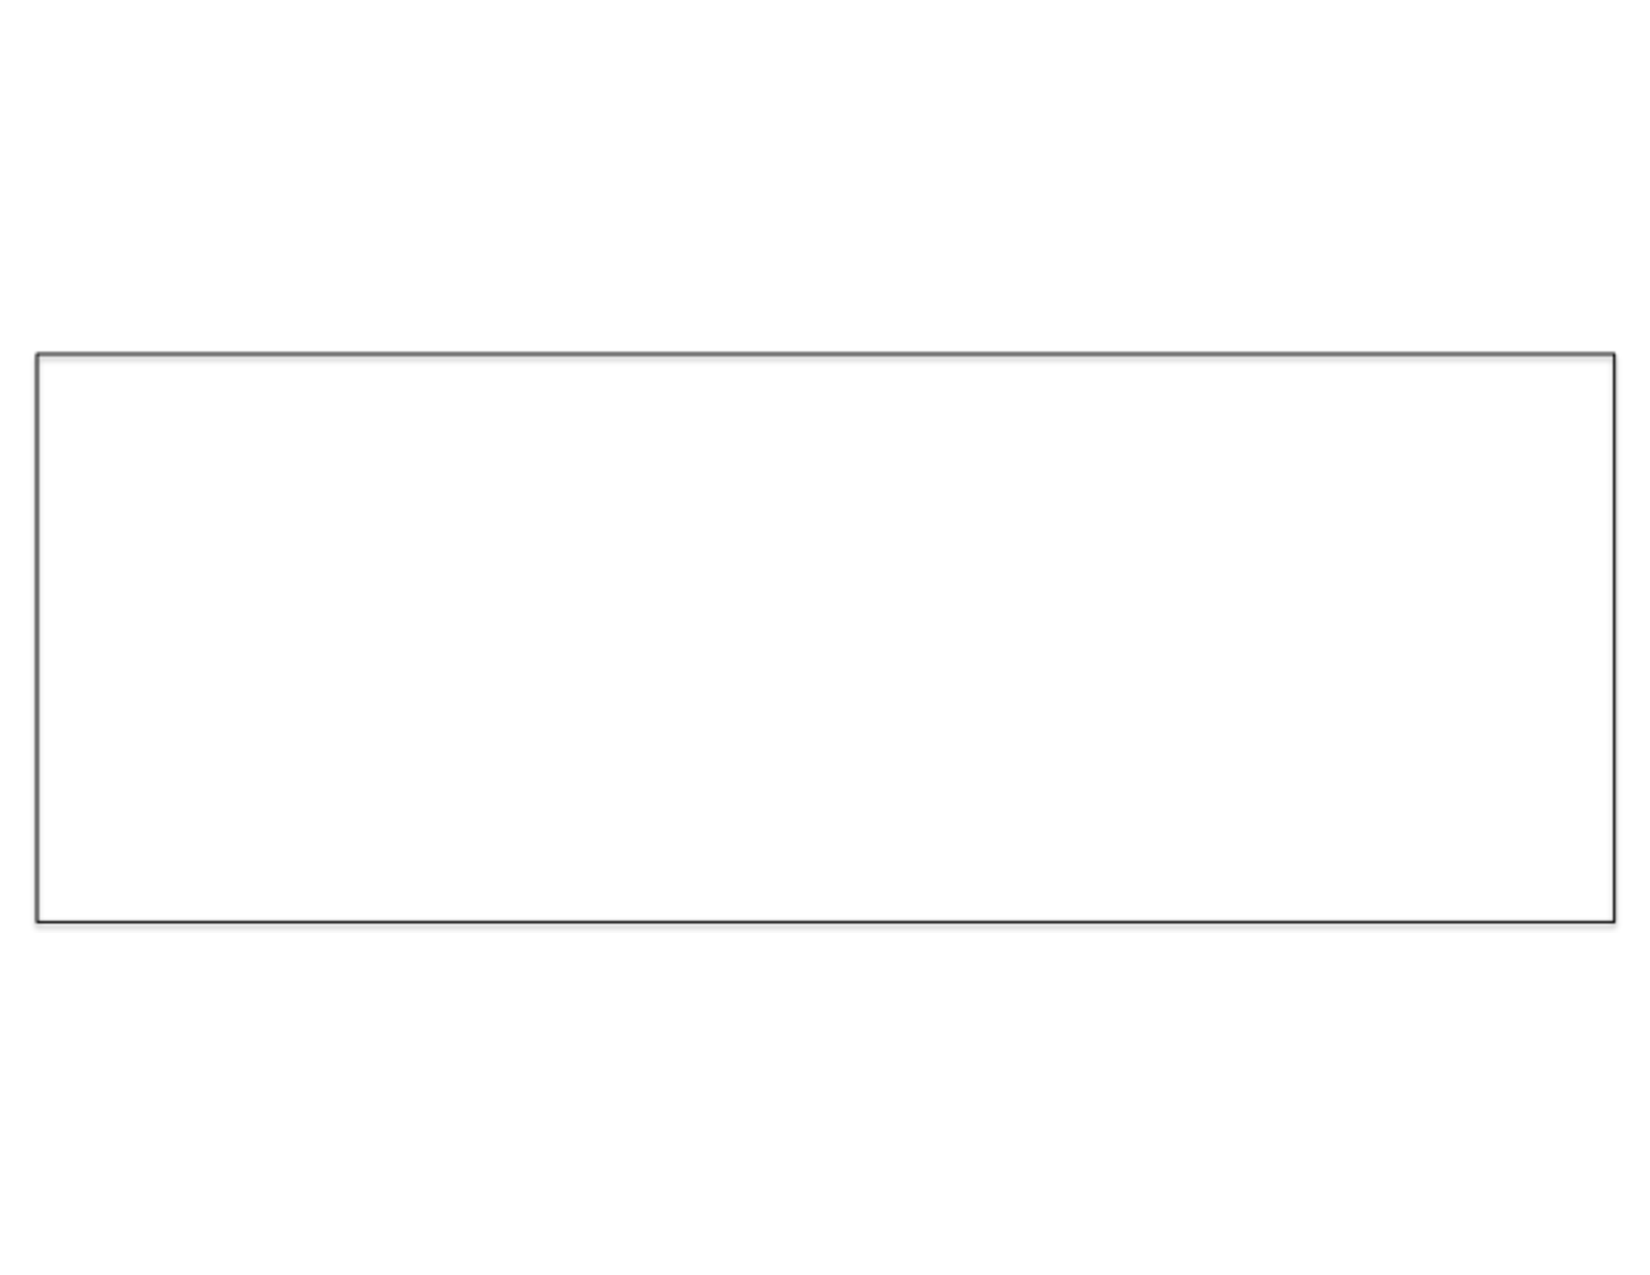
\includegraphics[scale=0.5]{figs/blankrectangle}
\caption{Gestures. Lorem Ipsum is simply dummy text of the printing and typesetting industry. Lorem Ipsum has 
been the industry's standard dummy text ever since the 1500s, when an unknown printer took a galley of 
type and scrambled it to make a type specimen book.  }
\label{fig:gestures}
\end{center}
\end{figure*}

\section{Setup and interaction}
Figure~\ref{fig:gestures} shows all the components of our architecture and the gestures used to interact with the system.  To
start we need to capture the objects and relationship between them.  Specifically, we set up the hierarchical organization of
objects with the building at the root, followed by \emph{spaces} and \emph{inventory} within the building, and data streams at the leaves.
The spaces subtree is the hierarchical organization of floors, rooms, and areas on those floors.  The inventory is a folder where
each of the physical objects is placed.  We used symbolic links to associate items in the inventory with the location
they are in.  In addition, we added a categorical subtree to ease aggregation with respect to the category of devices.
For personalized accounting, users created their own folder that points to items that belong to them.
Figure~\ref{fig:hierarchy} shows a partial view of the hierarchy that supports our applications.

After the hierarchy is constructed, we place QR codes on objects in the world and register them.  The registration process
for locations includes the following steps:

\begin{enumerate}
\item Place QR code somewhere in the space.
\item Scan QR code.
\item Choose which space it represents.
\end{enumerate}

\vspace{0.04in}

The basic set of spaces that initially inputted by hand are the building and the floors.  We placed QR code on the entrance of the building
and the main door to enter the floor.  Once each of these spaces is registered, the user can set their context by swipe the QR code tag.
When rooms are added, the user first scans the tag for the floor they are on, then they place a tag on the room and they enter information
about the room.  For items, the process is the same.  We scan the room we are in, place the tag on the object and enter information about
object.

The initial location scan sets the context.  For example, when you first enter a building, you scan the QR code associated with that building.
The {\tt URL} fetched from the QR code is first resolved.  This is an example {\tt URL} encoded in a QR code: {\tt http://tinyurl.com/6235eyw}.
When this is resolved, we get an empty response in the body, but we use the header to identify the QR code identifier that we associate
with the item.  The response header looks as follows:

\begin{figure}[htb!]
\begin{center}
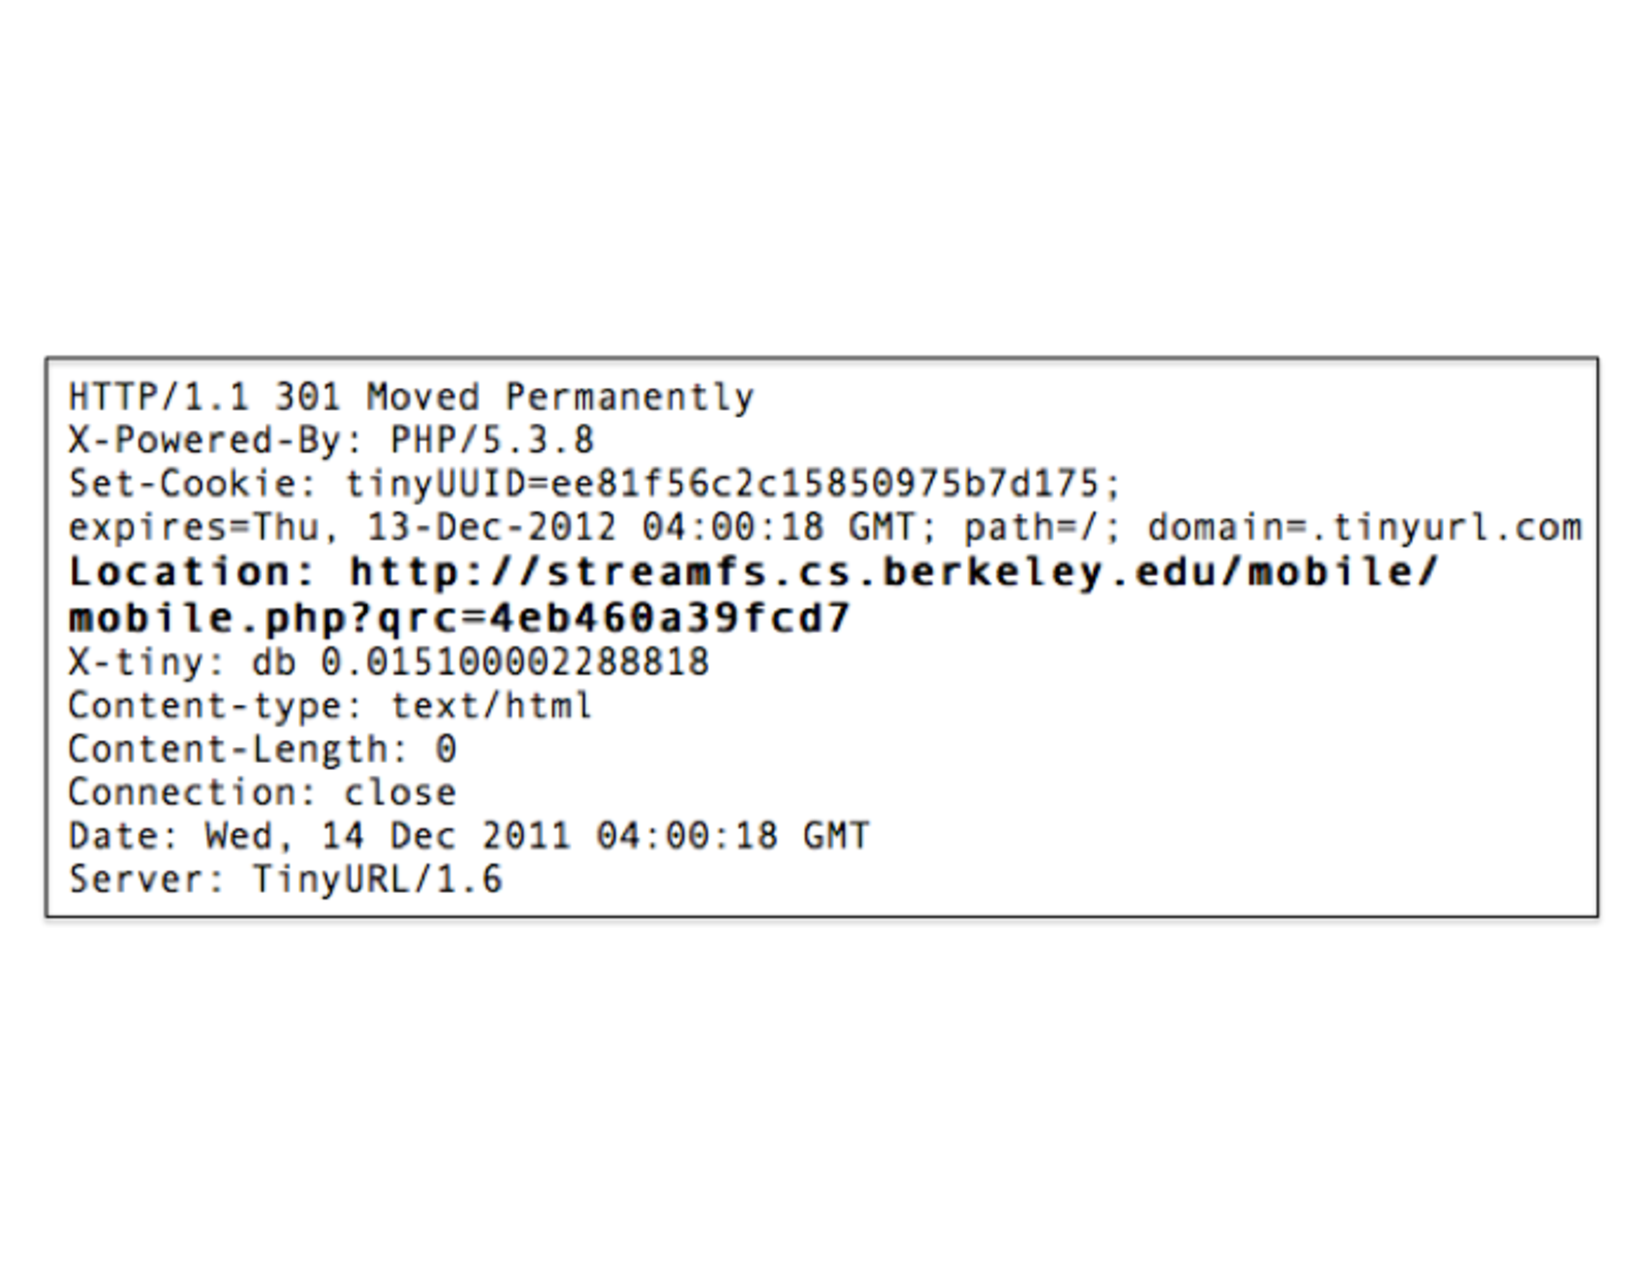
\includegraphics[scale=0.3]{figs/tinyurlhdr}
\caption{The header of the response from the {\tt tinyUrl} when resolving a QR code.  The `Location' attribute
is used to extract the unique identifier for the object this QR code tags.  It is also used to re-direct
users without the phone application to a meaningful web address for the object.}
\label{fig:qrcex}
\end{center}
\end{figure}

As previously mentioned, we designed our QR code with the minimal amount of information to minimize scanning time.  Therefore, we rely
on the network to give us the rest of the information.  This is a design choice.  Network connectivity is more reliable
than scanner quality, especially since we were dealing with a diverse set of phones and phones cameras of varying quality.
The QR code contains a tinyURL, which resolves to a longer URL.  The longers URL itself serve a dual purpose.  It provides 
a web address for users to re-direc to and find information and various read-only services for the object.  However, because
the {\tt URL} also contains a unqiue identifer \emph{qrc}, it can be used to provide for sophisticated services and capabilities.
An example is the ability to change the virtual structure of inter-relationship between this object and other objects.  This
is demonstrated in our energy auditing application discussed in detail in section~\ref{sec:eaudit}.
Once items are tagged, they can be added and removed by swiping the tag and pressing the button for what you want to do with
the item.  You also check into locations either explicit with a location-tag swipe or implicitly with an item swipe.

\subsection{Inter-relationship capture}
\label{sec:binding}
%Talking about how you bind an item and meter.
There is a special relationship between meters and items.  Items are attached to meters, but more importantly, the data
collected from the sensor \emph{represents} the underlying dynamics of some physical measurement related to the item.  A power 
meter attached to a television gives us the power profile of that television over some time period.  Furthermore, if the meter 
is removed
from the television and attached to another item, that change needs to be recorded, so that we do not attribute the power
trace from the second item to the television.  There are also items are that attached to each other that can affect how we 
aggregate feeds.  For example, in our deployment, we sometimes connect meters to power-strips, which have multiple items
attached to them.  The meter serves as a proxy-aggregate for the attached the power strip that's attached the meter.

%FILL IN WITH REAL GRAPH
\begin{figure}[htb!]
\begin{center}
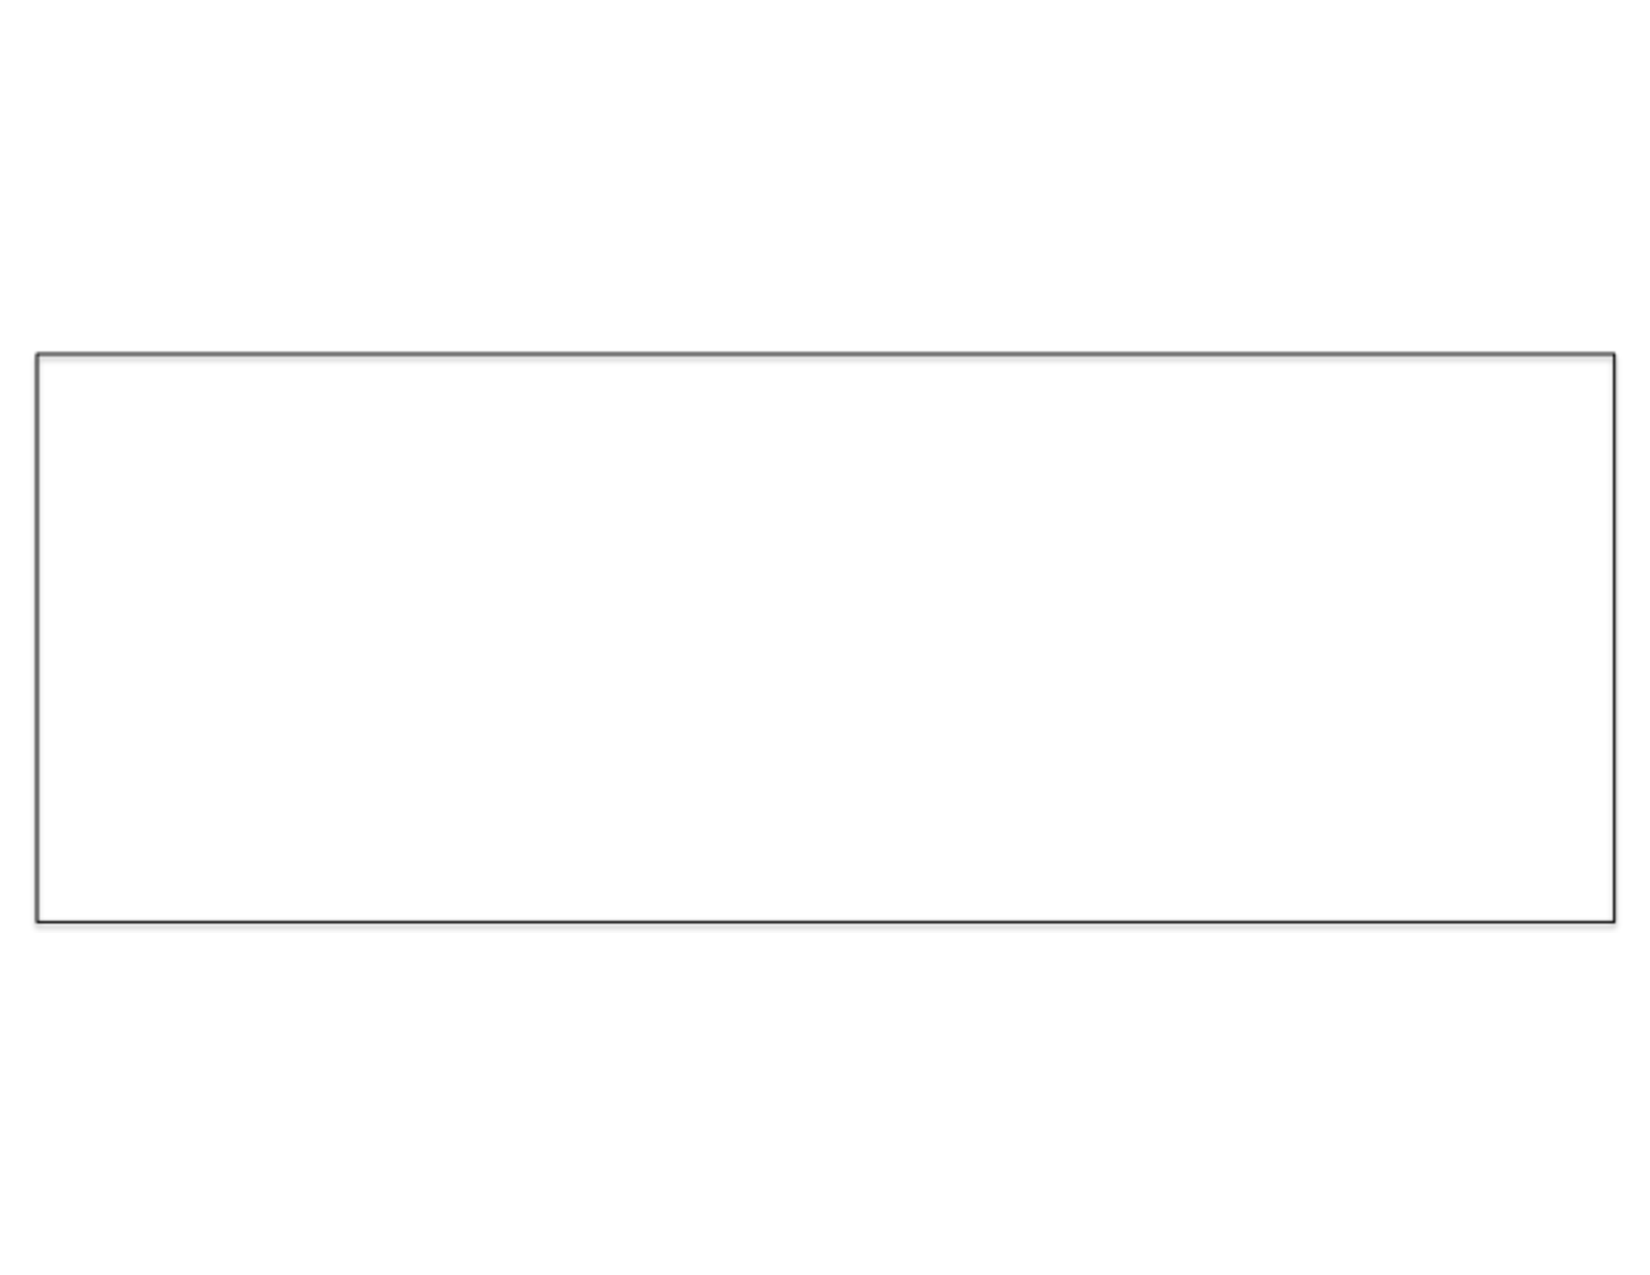
\includegraphics[scale=0.3]{figs/blankrectangle}
\caption{Attach and bind. Lorem Ipsum is simply dummy text of the printing and typesetting industry. Lorem Ipsum has 
been the industry's standard dummy text ever since the 1500s, when an unknown printer took a galley of 
type and scrambled it to make a type specimen book.  }
\label{fig:attachandbind}
\end{center}
\end{figure}

Both types of relationship are interpretted by how nodes are symbolically linked.  If a meter is the child
of an item, it is bound to that item and can be used as a proxy for measurements pertaining to that item.
If an item is a child of a meter, it is attached to the meter, but the measure is not taking measurements
pertaining to the item, instead if it taking measurement of the children of the item.  Figure~\ref{fig:attachandbind}
highlights the two kinds of relationships interpretted by our applications.  The one of the left shows
a bind relationship while the one of the right shows and attach relationship.
To bind or attach the gesture is the same.  You first swipe the item the swipe the meter and press a button to either
un/attach or un/bind.

% \begin{itemize}
% \item Hierarchical organization
% 	\begin{itemize}
% 	\item building
% 		\begin{itemize}
% 		\item spaces
% 		\item inventory
% 		\end{itemize}
% 	\item symbolic links between spaces and inventory
% 	\item categorical
% 	\item users
% 	\end{itemize}
% \item Setting virtual view -- construction of the world
% 	\begin{itemize}
% 	\item Add/Remove through scan and input
% 	\item Un/Attaching
% 	\item Un/Binding
% 	\end{itemize}
% \item Setting context -- where in the world am i
% 	\begin{itemize}
% 	\item Check-in swipe
% 	\item Swiping items
% 	\end{itemize}
% \end{itemize}







